% XeLaTeX can use any Mac OS X font. See the setromanfont command below.
% Input to XeLaTeX is full Unicode, so Unicode characters can be typed directly into the source.

% The next lines tell TeXShop to typeset with xelatex, and to open and save the source with Unicode encoding.

%!TEX TS-program = xelatex
%!TEX encoding = UTF-8 Unicode

\documentclass[11pt,twoside]{book}
\usepackage{multirow}
\usepackage{pdfpages}

\usepackage{geometry}                % See geometry.pdf to learn the layout options. There are lots.
%\usepackage[margin=1cm]{geometry}


%	\addtolength{\textwidth}{1.75in}
%
%	\addtolength{\topmargin}{-.875in}
%	\addtolength{\textheight}{1.75in}

\geometry{a4paper,left=20mm,top=20mm,total={162mm,230mm}}                   % ... or a4paper or a5paper or ... 
%\geometry{landscape}                % Activate for for rotated page geometry
%\usepackage[parfill]{parskip}    % Activate to begin paragraphs with an empty line rather than an indent

\setcounter{secnumdepth}{5}

\usepackage{amssymb}
%\usepackage{todonotes}
\setlength{\marginparwidth}{2cm}
\usepackage[backgroundcolor=white,bordercolor=blue,linecolor=blue,textwidth=1cm]{todonotes}
\usepackage{booktabs}
\usepackage{longtable}
\usepackage{url}

\usepackage[depth=4]{bookmark}


\usepackage{algorithm}
\usepackage{algpseudocode}

\usepackage{imakeidx}
\usepackage[utf8]{inputenc}
\usepackage[T1]{fontenc}
\makeindex[intoc]

\usepackage[font=normalsize]{caption}  

\usepackage{hyperref}
\hypersetup{
    colorlinks,
    citecolor=black,
    filecolor=black,
    linkcolor=black,
    urlcolor=black
}

\usepackage{xcolor}
\usepackage{listings}

\makeatletter
\global\let\tikz@ensure@dollar@catcode=\relax
\makeatother

\definecolor{mGreen}{rgb}{0,0.6,0}
\definecolor{mGray}{rgb}{0.5,0.5,0.5}
\definecolor{mPurple}{rgb}{0.58,0,0.82}
\definecolor{backgroundColour}{rgb}{0.95,0.95,0.92}
\definecolor{gray}{rgb}{0.4,0.4,0.4}
\definecolor{darkblue}{rgb}{0.0,0.0,0.6}
\definecolor{cyan}{rgb}{0.0,0.6,0.6}

\lstdefinestyle{CStyle}{
    backgroundcolor=\color{backgroundColour},   
    commentstyle=\color{mGreen},
    keywordstyle=\color{magenta},
    numberstyle=\tiny\color{mGray},
    stringstyle=\color{mPurple},
    basicstyle=\scriptsize\ttfamily,
    breakatwhitespace=false,         
    breaklines=true,                 
    captionpos=b,                    
    keepspaces=true,                 
    numbers=left,                    
    numbersep=5pt,                  
    showspaces=false,                
    showstringspaces=false,
    showtabs=false,                  
    tabsize=2,
    language=C
}


\lstset{ 
  backgroundcolor=\color{white},   % choose the background color; you must add \usepackage{color} or \usepackage{xcolor}; should come as last argument
  basicstyle=\footnotesize\ttfamily,        % the size of the fonts that are used for the code
  breakatwhitespace=false,         % sets if automatic breaks should only happen at whitespace
  breaklines=true,                 % sets automatic line breaking
  captionpos=b,                    % sets the caption-position to bottom
  commentstyle=\color{gray},    % comment style
  deletekeywords={...},            % if you want to delete keywords from the given language
  %escapeinside={\%*}{*)},          % if you want to add LaTeX within your code
  %extendedchars=true,              % lets you use non-ASCII characters; for 8-bits encodings only, does not work with UTF-8
  %firstnumber=1000,                % start line enumeration with line 1000
  frame=single,	                   % adds a frame around the code
  keepspaces=true,                 % keeps spaces in text, useful for keeping indentation of code (possibly needs columns=flexible)
  keywordstyle=\color{blue},       % keyword style
  language=C,                 % the language of the code
  %morekeywords={*,...},            % if you want to add more keywords to the set
  numbers=left,                    % where to put the line-numbers; possible values are (none, left, right)
  numbersep=5pt,                   % how far the line-numbers are from the code
  numberstyle=\tiny\color{gray}, % the style that is used for the line-numbers
  rulecolor=\color{black},         % if not set, the frame-color may be changed on line-breaks within not-black text (e.g. comments (green here))
  showspaces=false,                % show spaces everywhere adding particular underscores; it overrides 'showstringspaces'
  showstringspaces=false,          % underline spaces within strings only
  showtabs=false,                  % show tabs within strings adding particular underscores
  stepnumber=1,                    % the step between two line-numbers. If it's 1, each line will be numbered
  stringstyle=\color{black},     % string literal style
  tabsize=2,	                   % sets default tabsize to 2 spaces
}

\lstset{
  columns=fullflexible,
  showstringspaces=false,
  commentstyle=\color{gray}\upshape,
  backgroundcolor=\color{backgroundColour},   
  commentstyle=\color{mGreen},
  keywordstyle=\color{magenta},
  numberstyle=\tiny\color{mGray},
  stringstyle=\color{mPurple},
  basicstyle=\scriptsize\ttfamily,
  tabsize=2
}

\lstdefinelanguage{XML}
{
  morestring=[b]",
  morestring=[s]{>}{<},
  morecomment=[s]{<?}{?>},
  stringstyle=\color{black},
  identifierstyle=\color{darkblue},
  keywordstyle=\color{cyan},
  morekeywords={xmlns,version,type}% list your attributes here
}


% Will Robertson's fontspec.sty can be used to simplify font choices.
% To experiment, open /Applications/Font Book to examine the fonts provided on Mac OS X,
% and change "Hoefler Text" to any of these choices.

\renewcommand{\scriptsize}{\tiny}

\usepackage{fontspec,xltxtra,xunicode}
\defaultfontfeatures{Mapping=tex-text}
\setromanfont[Scale=MatchLowercase,Mapping=tex-text]{Optima}
\setsansfont[Scale=MatchLowercase,Mapping=tex-text]{Optima}
\setmonofont[Scale=MatchLowercase]{Andale Mono}

%%%% Graphics
\usepackage{graphicx}
\usepackage{tikz}
\definecolor{unilublue}{RGB}{55,149,218}
\definecolor{sntred}{RGB}{219,46,27}
\definecolor{sntpurple}{RGB}{86,30,130}
%\definecolor{sntblue}{RGB}{50,130,207}
\definecolor{sntblue}{RGB}{55,149,218}

\pgfdeclareimage[width=30mm]{logo-snt}{logos/logo-snt}
\pgfdeclareimage[width=30mm]{logo-uni-lu}{logos/logo-uni-lu}

%%%% Fancy
\usepackage{fancyhdr}

%%%% Increase page length
\addtolength{\textheight}{1in}

%%%% Sections
\usepackage{xspace}
\usepackage{sectsty}
\allsectionsfont{\sffamily}

\setlength{\parskip}{1em}

%\renewcommand{\,}{$^{\cdot}$}

%%%% Title
\newcommand{\titleone}{\textsf{D5}}
\newcommand{\titletwo}{\textsf{Evaluation of mutation testing process and methodology definition}}
\newcommand{\titlethree}{\textsf{}}

\newcommand{\todoinline}[1]{\todo[color=orange,inline]{ \textbf{TODO}: #1 }}

\newcommand{\TODO}[1]{\todo[color=orange,inline]{ \textbf{TODO}: #1 }}
\newcommand{\DONE}[1]{\todo[color=green,inline]{ \textbf{DONE}: #1 }}


\usepackage{amsmath}
\usepackage{array}
\usepackage{lipsum}

\usepackage{algorithm}
\usepackage{algpseudocode}

\newcommand{\LXS}{LXS\xspace{}}
\newcommand{\GSL}{GSL\xspace{}}
\newcommand{\ESA}{ESA\xspace{}}
\newcommand{\ESAIL}{ESAIL\xspace}
\newcommand{\PARAM}{LIBPARAM\xspace}
\newcommand{\UTIL}{LIBUTIL\xspace}

\newcommand{\GomSpace}{GomSpace\xspace}
\newcommand{\LuxSpace}{LuxSpace\xspace}
\newcommand{\ONE}{GSL\xspace}
\newcommand{\TWO}{LXS\xspace}
\newcommand{\CITONE}{~\cite{GSL}}
\newcommand{\CITTWO}{~\cite{LXS}}
\newcommand{\LAUNCH}{on September 2020~\cite{ESAILlaunch}}
\newcommand{\OPENCSP}{the open source CubeSat Space Protocol (\CSP) library~\cite{CSP}}


\newcommand{\ADCS}{\emph{\ESAIL-ADCS}\xspace}
\newcommand{\GPS}{\emph{\ESAIL-GPS}\xspace}
\newcommand{\PDHU}{\emph{\ESAIL-PDHU}\xspace}
\newcommand{\SVF}{\emph{\ESAIL-SVF}\xspace}

\newcommand{\FIXME}[1]{#1}

\newcommand{\CHANGED}[1]{\textcolor{black}{#1}}
\newcommand{\CHANGEDTWO}[1]{\textcolor{black}{#1}}
\newcommand{\CHANGEDOCT}[1]{\textcolor{black}{#1}}
\newcommand{\CHANGEDNOV}[1]{\textcolor{black}{#1}}

\newcommand{\TRFOUR}[1]{\textcolor{green}{#1}}

\newcommand{\STARTCHANGEDNOV}{\color{black}}
\newcommand{\ENDCHANGEDNOV}{\color{black}}

\newcommand{\STARTCHANGEDWPT}{\color{black}}
\newcommand{\ENDCHANGEDWPT}{\color{black}}


%\newcommand{\MREVISION}[2]{\todo{\tiny{#1}}\textcolor{blue}{#2}}
\newcommand{\MREVISION}[2]{#2}

%\newcommand{\REVTWO}[2]{\todo[color=red]{\tiny{#1}}\textcolor{red}{#2}}
\newcommand{\REVTWO}[2]{#2}

\newcommand{\REVNOV}[2]{\textcolor{black}{#2}}

\newcommand{\REVOCT}[2]{\todo{\tiny{#1}}\textcolor{blue}{#2}}
\newcommand{\REVTOOL}[2]{\todo{\tiny{#1}}\textcolor{blue}{#2}}

\newcommand{\EMPH}[1]{\textbf{\emph{#1}}}
\newcommand{\INDEX}[1]{\index{\MakeLowercase{#1}}\EMPH{#1}}

\newcommand{\APPR}{\emph{SMTS}\xspace}

\begin{document}

\pagestyle{fancy}
\renewcommand{\sectionmark}[1]{\markright{\textit{#1}}}

\renewcommand{\headrulewidth}{2pt}% 2pt header rule
\renewcommand{\headrule}{\hbox to\headwidth{%
  \color{sntblue}\leaders\hrule height \headrulewidth\hfill}}

\fancyhf{}

%\lhead{\fancyplain{}{\setlength{\unitlength}{1mm}
%\begin{picture}(0,0)
%\put(0,-4){
\includegraphics[width=50pt]{logos/logo-snt}}
%\end{picture}}} 

\newcommand{\DOCUMENTID}{ITT-1-9873-ESA-FAQAS-D5}
\lhead{\fancyplain{}{\textit{\DOCUMENTID}}}
\rhead{\fancyplain{}{\rightmark }}

\fancyfoot[C]{%
\begin{tikzpicture}[remember picture,overlay]
\path [fill=sntred]    ([xshift=88pt,yshift=20pt]current page.south west) rectangle
                       ([xshift=229pt,yshift=30pt] current page.south west);
\path [fill=sntpurple] ([xshift=229pt,yshift=20pt] current page.south west) rectangle
                       ([xshift=370pt,yshift=30pt] current page.south west);
\path [fill=sntblue]   ([xshift=370pt,yshift=20pt] current page.south west) rectangle
                       ([xshift=510pt,yshift=30pt] current page.south west);
\end{tikzpicture}
}

\fancyfoot[RO]{
\begin{tikzpicture}[remember picture,overlay]
\node [circle, ultra thick, fill=white, draw=sntblue] at ([xshift=530pt,yshift=35pt] current page.south west) {\thepage};
\end{tikzpicture}}

\fancyfoot[LE]{
\begin{tikzpicture}[remember picture,overlay]
\node [circle, ultra thick, fill=white, draw=sntblue] at ([xshift=65pt,yshift=35pt] current page.south west) {\thepage};
\end{tikzpicture}}

\newcommand{\JMR}[2]{\textcolor{black}{#2}}
\newcommand{\NEWFSCI}[1]{\textcolor{black}{#1}}

\newcommand{\JMRCHANGE}[1]{\textcolor{black}{#1}}
\newcommand{\UPDATE}[1]{\textcolor{black}{#1}}

\newcommand{\SAIL}{\emph{ESAIL}\xspace}
\newcommand{\MLFS}{\emph{MLFS}\xspace}
\newcommand{\GCSP}{\emph{LIBGCSP}\xspace}

\newcommand{\MPTS}{\emph{MASS-reduced} test suite\xspace}
\newcommand{\MPTSs}{\emph{MASS-reduced} test suites\xspace}
\newcommand{\ExaE}{ExactEarth}

\newcommand{\prog}{P}
\newcommand{\prop}{}




\thispagestyle{empty}

\begin{tikzpicture}[remember picture,overlay]
\path [fill=sntred]    ([xshift=30pt,yshift=20pt]current page.south west) rectangle
                       ([xshift=210pt,yshift=50pt] current page.south west);
\path [fill=sntpurple] ([xshift=210pt,yshift=20pt] current page.south west) rectangle
                       ([xshift=390pt,yshift=50pt] current page.south west);
\path [fill=sntblue]   ([xshift=390pt,yshift=20pt] current page.south west) rectangle
                       ([xshift=570pt,yshift=51pt] current page.south west);
\path [fill=unilublue] ([xshift=30pt,yshift= 50pt] current page.south west) --
                       ([xshift=570pt,yshift= 50pt] current page.south west)
                       [rounded corners=20pt] --
                       ([xshift=570pt,yshift=740pt] current page.south west)
                       [sharp corners] --
                       ([xshift=30pt,yshift=740pt] current page.south west);
\node [fill=white,rounded corners=0pt,inner xsep=6pt,inner ysep=3pt]
      at ([xshift=523pt,yshift=120pt] current page.south west)
      {\pgfuseimage{logo-uni-lu}};

\node [fill=white,rounded corners=2pt,inner xsep=6pt,inner ysep=3pt]
      at ([xshift=520pt,yshift=780pt] current page.south west)
      {\pgfuseimage{logo-snt}};

%\node [circle, fill=white, draw=sntblue] at ([xshift=550pt,yshift=35pt] current page.south west) {a};

\node[draw=none,fill=none,right] at (-1, -7){\color{white}\LARGE\bf\titleone};
\node[draw=none,fill=none,right] at (-1, -8){\color{white}\LARGE\bf\titletwo};
\node[draw=none,fill=none,right] at (-1, -9){\color{white}\LARGE\bf\titlethree};

\node[draw=none,fill=none,right] at (-1, -12){\color{white}\Large\textsf{O. Cornejo, F. Pastore, E. Viganò}};
\node[draw=none,fill=none,right] at (-1, -13){\color{white}\Large\textsf{Interdisciplinary Centre for Security, Reliability and Trust}};
\node[draw=none,fill=none,right] at (-1, -14){\color{white}\Large\textsf{University of Luxembourg}};
\node[draw=none,fill=none,right] at (11, -16){\color{white}\textsf{ITT-1-9873-ESA-FAQAS-SUTP}};
\node[draw=none,fill=none,right] at (11, -17){\color{white}\Large\textsf{Issue 4, Rev. 1}};
\node[draw=none,fill=none,right] at (11, -18){\color{white}\Large\textsf{\today}};
\node[draw=none,fill=none,right] at (-1, -24){\color{white}\tiny\textsf{EUROPEAN SPACE AGENCY. CONTRACT REPORT.}};
\node[draw=none,fill=none,right] at (-1, -24.3){\color{white}\tiny\textsf{The work described in this report was done under ESA contract. Responsibility for the contents resides in the author or organisation that prepared it.}};
\node[draw=none,fill=none,right] at (-1, -24.8){\color{white}\tiny\textsf{The copyright in this document is vested in the University of Luxembourg.}};
\node[draw=none,fill=none,right] at (-1, -25.1){\color{white}\tiny\textsf{This document may only be reproduced in whole or in part, or stored in a retrieval system,or transmitted in any form, or by any means electronic,}};
\node[draw=none,fill=none,right] at (-1, -25.4){\color{white}\tiny\textsf{mechanical, photocopying or otherwise, either with the prior permission of the University of Luxembourg or in accordance with the terms of ESTEC Contract No. 4000128969/19/NL/AS.}};

\node[draw=none,fill=none,right] at (-1, -24){\color{white}\tiny\textsf{EUROPEAN SPACE AGENCY. CONTRACT REPORT.}}; 
\node[draw=none,fill=none,right] at (-1, -24.3){\color{white}\tiny\textsf{The work described in this report was done under ESA contract. Responsibility for the contents resides in the author or organisation that prepared it.}};
\node[draw=none,fill=none,right] at (-1, -24.8){\color{white}\tiny\textsf{The copyright in this document is vested in the University of Luxembourg.}};
\node[draw=none,fill=none,right] at (-1, -25.1){\color{white}\tiny\textsf{This document may only be reproduced in whole or in part, or stored in a retrieval system,or transmitted in any form, or by any means electronic,}}; 
\node[draw=none,fill=none,right] at (-1, -25.4){\color{white}\tiny\textsf{mechanical, photocopying or otherwise, either with the prior permission of the University of Luxembourg or in accordance with the terms of ESTEC Contract No. 4000128969/19/NL/AS.}};


\end{tikzpicture}

\newpage


% !TEX root = MAIN.tex

\section*{Revisions}
\label{sec:revisions}


\setlength\LTleft{0pt}
\setlength\LTright{0pt}
\tiny 
%@{\extracolsep{\fill}}
\begin{longtable}{|p{2cm}|p{1cm}|p{1.5cm}|p{9cm}|@{}}
\label{table:codeoperators} \\
\hline
\textbf{Issue Number}&\textbf{Date}&\textbf{Authors}&\textbf{Description}\\
\hline
ITT-1-9873-ESA-FAQAS-FR
Issue 1 Rev. 1&
October 29th, 2021&
Fabrizio Pastore, Oscar Cornejo, Enrico Viganò&
\begin{minipage}{8cm}
Initial release.
\end{minipage}
\\
\hline
ITT-1-9873-ESA-FAQAS-FR
Issue 1 Rev. 2&
November 11th, 2021&
Fabrizio Pastore, Oscar Cornejo, Enrico Viganò&
\begin{minipage}{8cm}
Added Chapter~\ref{chap:deliverables_summary} (deliverables summary).\\
Added Chapter~\ref{ch:toolset} (description of toolset package).\\
Added information about input and outputs of the tools in Chapter~\ref{chapter:methodology} (see blue text).
\end{minipage}
\\
\hline
                                                    
\end{longtable}
\normalsize

\clearpage

% !TEX root = MAIN.tex

\section*{Delivered Items}
\label{sec:deliverables}

In the following Table we provide a list of deliverable items released with this document. Each Item is identified by it's path on the Alfresco system.

\setlength\LTleft{0pt}
\setlength\LTright{0pt}
\tiny 
%@{\extracolsep{\fill}}
\begin{longtable}{|p{9cm}|p{6cm}@{}}
\label{table:deliverables} \\
\hline
\textbf{Deliverable}&Description\\
\hline
ASN1CC-CaseStudy/Specifications/ACN-UM-v-3-2.pdf&User manual of ASN1 Compiler\\
ASN1CC-CaseStudy/Specifications/taste-documentation-current.pdf&Taste software documentation including ASN1 overview\\
\hline
GSL-CaseStudies/Specifications/gs-man-nanosoft-ms100-command-and-management-sdk-3.6.2-1-g67fe6e1.pdf&LXS softwrae specifications\\
\hline
LXS-CaseStudies/Specifications&Folder with LXS specifications\\
LXS-CaseStudies/Specifications/FAQAS-LXS-MAN-001\_1- SVF Software Installation and User Manual.pdf&SVF and ESAIL Software Installation and User Manual\\
LXS-CaseStudies/Specifications/ESAIL-LXS-ICD-P-0184\_2A ADCS IF SW External ICD.docx&\\
LXS-CaseStudies/Specifications/ESAIL-LXS-SDD-P-0105\_1B On-board Application Software Design Document&\\
LXS-CaseStudies/Specifications/MOC-applicable MIB egos-mcs-s2k-icd-0001-version7.0-FINAL&SCOS-2000 Database Import ICD\\
LXS-CaseStudies/Specifications/ocp.dat&SCOS-2000 Database file containing the specifications of the nominal value ranges for ESAIL ADCS parameters.\\
\hline
SnT-Software/FAQAS-DataDrivenMutator-Buffers.zip&Preliminary implementation of the data-driven mutation testing component\\
%\begin{minipage}{8cm}
%Initial release.
%\end{minipage}
\\
\hline

%ITT-1-9873-ESA-FAQAS-D1
%Issue 4
%&DATE
%&Fabrizio Pastore, Oscar Cornejo
%&
%\begin{minipage}{8cm}
%\end{minipage}
%\\

%\hline
                                                    
\end{longtable}
\normalsize

\clearpage



\tableofcontents



% !TEX root = MAIN.tex

\chapter{Scope and content}

This document is the deliverable SSS of the ESA activity ITT-1-9873-ESA. It concerns requirements specification for the \emph{FAQAS framework} to be delivered by ITT-1-9873-ESA. Following the structure described in the SoW \emph{AO9873-ws00pe\_SOW.pdf}, it provides the structured requirements baseline for the FAQAS framework according to ECSS-E-ST-40C Annex B.
 
\section{Applicable and reference documents}

\begin{itemize}
\item{D1 - Mutation testing survey}
\item{D2 - Study of mutation testing applicability to space software}
\end{itemize}

\chapter{Terms, definitions and abbreviated terms}

\begin{itemize}
\item{FAQAS}: activity ITT-1-9873-ESA
\item{FAQAS-framework}: software system to be released at the end of WP4 of FAQAS
\item{D2}: Deliverable D2 of FAQAS, \emph{Study of mutation testing applicability to space software}
\item{KLEE}: Third party test generation tool, details are provided in D2.
\item{SUT}: Software under test, i.e, the software that should be mutated by means of mutation testing.
\item{WP}: Work package
\end{itemize}

\clearpage
 



% !TEX root = MAIN.tex

\section{Acronyms and Abbreviations}
\label{sec:acronyms}


%@{\extracolsep{\fill}}
\begin{tabular}{|p{1.5cm}|p{14.5cm}|}
%&\TODO{Add acronyms. OSCAR: I've add some...} \\

%ACO & Ant Colony Optimization\\
D1& Deliverable 1 of FAQAS activity, \emph{Analysis and Survey of Mutation Testing}\\
D2& Deliverable 2 of FAQAS activity, \emph{Study of Mutation Testing Applicability to Space Software}\\
FOM & First Order Mutant\\
HOM & Higher-Order Mutant\\
LOC & Lines of Code\\
%SBST & Search Based Software Testing\\
%Fabrizio: we cannot use SE as acronym
%SE & Symbolic Execution\\
SOM & Second Order Mutant\\
SUT & Software Under Test\\
TS & Test Suite\\
UL HPC & University of Luxembourg High Performance Computing

%Comment #2:
%When generating the pdf file, make sure to have the index of the document on the left, so that the document is easier to navigate.
%Author: Pedro Barrios Subject: Sticky Note Date: 28/02/2020, 09:18:06
%Comment #3:
%Try to make the document a bit more friendly to read (e.g. by adding some sentences in bold (see the highlighted ones for this paragraph), making bigger
%separation between paragraphs, ...)
%Author: Pedro Barrios Subject: Sticky Note Date: 28/02/2020, 09:18:11
%Comment #4:
%It is perhaps interesting to add a chapter with some basic definitions?
%e.g. equivalent mutant, redundant mutant, mutation score, killed mutant, live mutant, weak mutation, ...
%Author: Pedro Barrios Subject: Sticky Note Date: 28/02/2020, 09:18:18
%Comment #5:
%Please, consider to add more examples.

                                                           
\end{tabular}
\normalsize

\clearpage

% !TEX root = MAIN.tex

\chapter{FAQAS Methodology}
\label{chapter:methodology}

FAQAS led to the development of a toolset that includes the following components:
\begin{itemize}
\item MASS (Mutation Analysis for Space Software), a tool that automatically executes code-driven mutation analysis. Code-driven mutation analysis consists of automatically generating mutants by altering the source code of the software under test. MASS implements a pipeline that makes it feasible in the context of space software. 
\item DAMAt (DAta-driven Mutation Analysis with Tables), a tool that automatically executes data-driven mutation analysis. Data-driven mutation analysis is an approach newly defined within FAQAS, which, instead of mutating the implementation of the software under test, alters the data exchanged by software components. Data-driven mutation analysis enables the injection of faults that affect simulated components (e.g., sensors), which is not feasible with traditional, code-driven mutation analysis.
\item SEMuS (Symbolic Execution-based MUtant analysis for Space software), a tool that automatically generates test inputs based on code-driven mutation analysis results. 
\item DAMTE, a methodology supported by the KLEE symbolic execution engine, for the generation of test inputs based on data-driven mutation analysis results.
\end{itemize}

\begin{figure}[tb]
\begin{center}
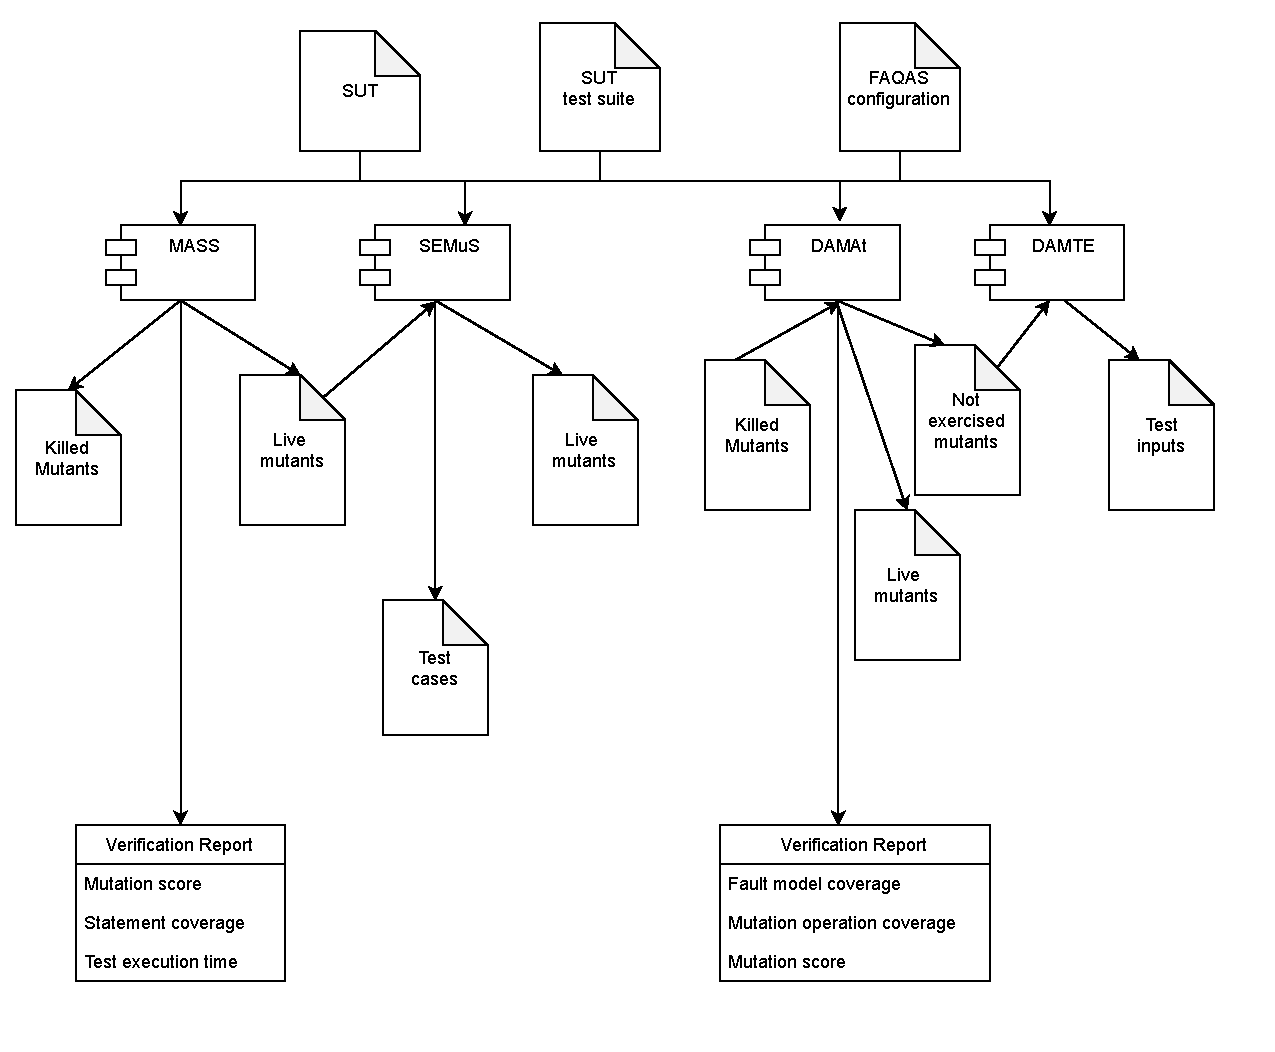
\includegraphics[width=0.8\textwidth]{images/FAQAS.drawio.pdf}
\caption{Overview of the FAQAS toolset}
\label{fig:FAQAS:toolset}
\end{center}
\end{figure}

Figure~\ref{fig:FAQAS:toolset} provides an overview of the input and outputs of the FAQAS toolset. All the components take as input the software under test (SUT), its test suite, and a set of configuration files. 
MASS generates as output a set of live mutants (i.e., mutants that do not lead to a test suite failure), a set of killed mutants (i.e., mutants that do not lead to a test suite failure), and information useful to draft a verification report, which includes the statement coverage of the SUT test suite, the mutation score, and the execution time of test cases.
SEMuS takes as input the list of live mutants detected by MASS and aims to generate test cases that kill them. After the
 execution of SEMuS, engineers have a set of additional test cases to be integrated into the SUT test suite and a list of live mutants (i.e., mutants for which SEMuS was not able to identify test inputs killing them). Live mutants shall be manually inspected by engineers to either determine if they are equivalent mutants or to manually derive a test input killing them.
 DAMAt generates as output a set of killed mutants (i.e., mutants that, during testing, successfully alter the data, and lead to test case failures), a set of live mutants (i.e., mutants that, during testing, successfully alter the data, but do not lead to test case failures), and a set of not executed mutants (i.e., mutants that, during testing, could not alter any data because the data they target is never exercised by the SUT); also, it provides information useful to draft a verification report, which includes the fault model coverage, the mutation operation coverage, and the mutation score.
 DAMTE is a manual procedure supported by the KLEE toolset that enables an engineer to automatically derive inputs that increase the fault model coverage and the mutation operation coverage.

In the following, we describe how the results generated by the FAQAS toolset enable the assessment and improvement of a test suite.
We focus on the fully automated tools, that is, MASS, DAMAt, and SEmuS.


\section{Code-driven Mutation Analysis: MASS}
\label{sec:meth:mass} 
 
Code-driven Mutation Analysis shall be performed by applying the MASS toolset following the setup procedures described in the SUM. 
At a high-level, the engineer needs to make the following choices
\begin{itemize}
\item Select the source files to mutate. Generally, all the source files of the SUT shall be considered for mutation. If the test suite targets only a subset  of files, the engineer can focus on that subset.
\item Select the sampling strategy. If the test suite of the SUT takes more than one hour to be executed, we suggest to rely on the \emph{FSCI} mutant sampling strategy. Otherwise, engineers can execute all the mutants (i.e., set \emph{sampling=NO})
\item Enable test suite reduction and prioritization. This choice enables MASS to further reduce test execution time by executing only a portion of the selected test cases based on statement coverage (see D2). In case of system test suites testing an SUT with multiple tasks running in parallel we suggest to avoid reducing the test suite.
\end{itemize}

For the other configuration parameters of MASS, the default options are generally appropriate for most of the SUTs.

The main output of MASS is a file named \emph{MASS\_RESULTS}, which includes the metrics listed in Table~\ref{table:mass:metrics}.
Three additional relevant output files generated by MASS are \emph{filtered\_live}, \emph{useful\_list\_a} and \emph{useful\_list\_b}. They contain the names of the live mutants (i.e., the ones not killed by the test suite).

\begin{table}[h]
\caption{}
\label{MASS Metrics}
\center
\begin{tabular}{|
@{\hspace{1pt}}p{120mm}|
}
\hline
\textbf{Metric name}\\
\hline
Number of mutants generated \\
%Mutants generation time&No\\
%Number of compiled mutants&No\\
%Percentage of compiled mutants&No\\
%Mutants compilation time&No\\
Number of mutants filtered using compiler optimisations \\
Sampling type \\
Number of mutants executed \\
%Number of test cases executed&No\\
%Test cases execution time \\
%Mutation execution traces \\
Number of killed mutants \\
Number of live mutants \\
Number of likely equivalent mutants \\
MASS mutation score \\
%List of useful mutants \\
Number of statements covered \\
Statement coverage \\
Minimum lines covered per source file \\
Maximum lines covered per source file \\
%Distribution of test cases exercising each statement&No\\
\hline
\end{tabular}
\end{table}

Within file \emph{MASS\_RESULTS}, the first metric to be inspected is the \emph{Statement coverage} (i.e., the percentage of statements being covered). Since MASS generates mutants only for the statements being exercised by the test suite, a high mutation score in the presence of a low statement coverage cannot indicate that the test suite has high quality. In general, we assume that engineers apply MASS to test suites that have already achieved the required quality level, according to ECSS practice (e.g., statement coverage of 100\%). The statement coverage shall thus simply enable engineers to determine if the test suite is correctly executed through MASS (i.e., if the statement coverage generated by MASS matches the expected one). The second metric to be inspected is the \emph{MASS mutation score}. It provides an indication of the quality of the test suite based on mutation analysis. According to literature, it shall be above 75\% otherwise the test suite shall be improved by introducing additional test cases. 


The next step is the \EMPH{improvement of the test suite}. This is performed by deriving test inputs that kill live mutants. 
To this end, engineers shall inspect all the mutants appearing in the file \emph{useful\_list\_a}. For each mutant, the engineer shall implement a test case capable of killing the mutant (i.e., a test case that fails with the mutant but not with the original software). 
The file \emph{useful\_list\_a} provides a list of mutants that are likely non redundant with each other because when tested by the SUT test suite they lead to a statement coverage profile (i.e., the set of statements covered during their execution) that differs. 
The file \emph{useful\_list\_b} provides a list of mutants that are likely redundant with the ones appearing in the file \emph{useful\_list\_a}; therefore the mutants listed in the file \emph{useful\_list\_b} will be likely killed by test cases implemented to kill the mutants in \emph{useful\_list\_a}.
The mutants within file \emph{useful\_list\_a} are sorted according to their diversity (i.e., the mutants on top are likely very different from each other. 
The file \emph{filtered\_live} provides the whole list of live mutants, that is the union of the mutants appearing in the files
\emph{useful\_list\_a} and \emph{useful\_list\_b}.

In general, since a same test case may kill more than one mutant, we suggest to derive test inputs for a subset of the mutants in \emph{useful\_list\_a} and then rerun the mutation analysis process. When rerunning the mutation analysis process, engineers shall focus the mutation analysis on the mutants appearing in \emph{useful\_list\_a} and in \emph{useful\_list\_b}. This is done by re-executing mutation analysis from step 6 (\emph{Execute mutants}), after replacing the mutant names in file \texttt{\$MASS\_WORKSPACE/COMPILED/all\_filtered} by the mutant names of list \emph{useful\_list\_a} and \emph{useful\_list\_b}.

When automated test generation with SEMuS is feasible; we suggest to rely on SEMuS to automatically generate test cases for all the mutants appearing in \emph{useful\_list\_a} and in \emph{useful\_list\_b} (see Section~\ref{sec:meth:semus}). 

When identifying inputs that kill mutants (either manually or with SEMuS) engineers may detect equivalent mutants. Equivalent mutants shall be removed from the list of mutants considered for the analysis.

If mutation analysis has been performed through mutants sampling (e.g., with \emph{FSCI}), after test suite improvement (i.e., after introducing test cases that kill all the mutants in \emph{useful\_list\_a} and in \emph{useful\_list\_b}), it is necessary to re-run mutation analysis to determine the mutation score of the improved test suite.


\section{Code-driven Mutation Testing: SEMuS}
\label{sec:meth:semus}

Figure~\ref{fig:semus_architecture} provides the workflow of SEMuS; it has been described in D2. The list of live mutants processed by SEMuS coincides with the list of mutants appearing in the file \emph{filtered\_live} presented in Section~\ref{sec:meth:mass}. 

The mutants for which SEMuS does not generate a test case (i.e., the corresponding output folder inside \emph{direct/TEMPLATE/FAQAS\_SEMu-out/produced-unittests} is empty) shall be manually inspected by engineers to determine if they are equivalent to the original software.

The test cases generated by SEMuS can instead be integrated as a regression test suite according to the \EMPH{test suite augmentation} procedure described in D2. Otherwise, engineers can copy the source code of the generated test cases inside the test suite of the SUT and add assertions according to the expected output generated by SEMuS (i.e., files \emph{.expected}, according to D2).

\begin{figure}[h]
\begin{center}
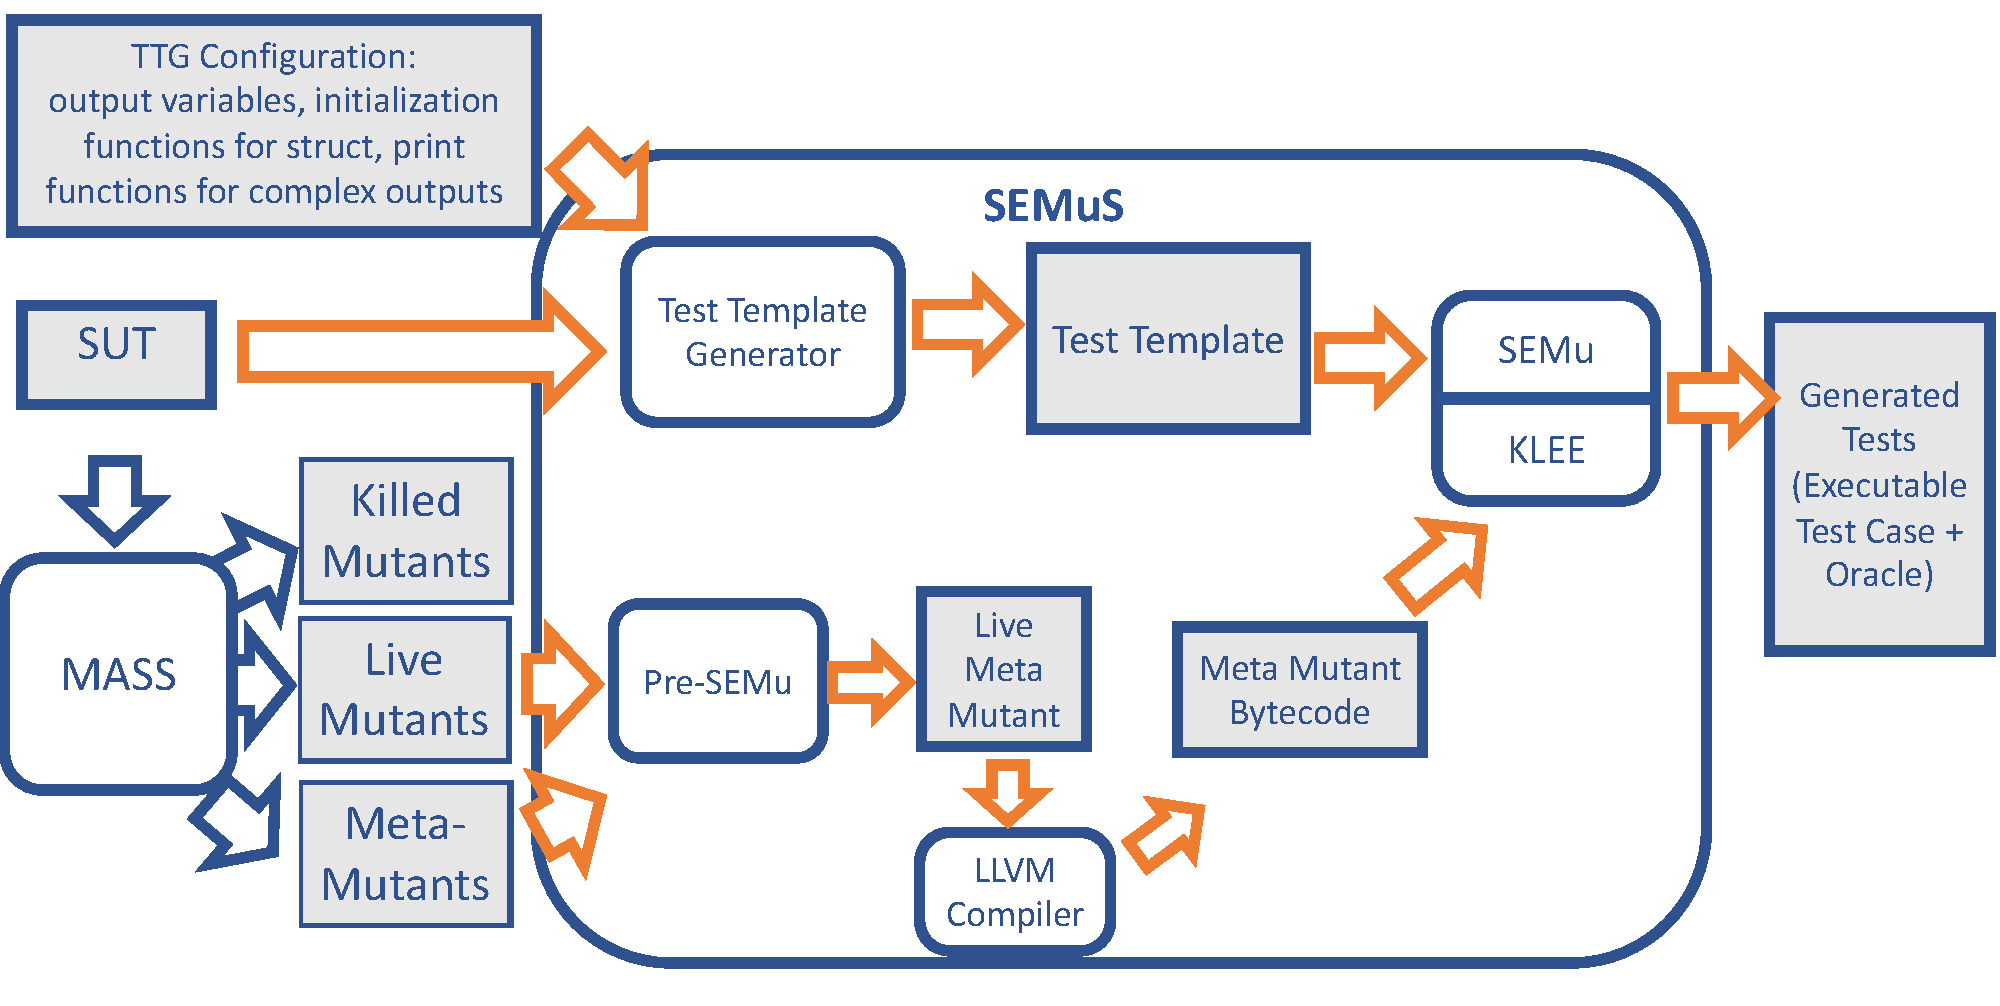
\includegraphics[width=0.8\textwidth]{images/semus-architecture2}
\caption{FAQAS-SEMuS Architecture and Workflow}
\label{fig:semus_architecture}
\end{center}
\end{figure}

\section{Data-driven Mutation Analysis: DAMAt}
\label{sec:meth:damat}

DAMAt shall be configured and applied according to the procedure describe in D2.
After the execution, DAMAt generates two files: \emph{final\_mutants\_table.csv} and \emph{mutation\_sum\_up.csv}.
The latter provides a high-level perspective on the results of the procedure, because it contains the three metrics defined in D2:
\begin{enumerate}
\item Fault model coverage, the percentage of fault models covered by the test suite.
\item Mutation operation coverage, the percentage of data items that have been mutated at least once, considering only those that belong to the data buffers covered by the test suite.
\item Mutation Score, the percentage of mutants killed by the test suite (i.e., leading to at least one test case failure) among the mutants that target a fault model and for which at least one mutation operation was successfully performed.
\end{enumerate}
 

A low score in one of the metrics indicate one of following scenarios, repsectively:
\begin{enumerate}
\item The message type targeted by a fault model is never exercised.
\item The message type is covered by the test suite, but it is not possible to perform some of the mutation operations. It depends on the fact that not all the input partitions are exercised by the test suite.
\item The mutation is performed but the test suite does not fail. It may depend on two reasons: (1) the test oracles are imprecise (e.g., they do not verify all the state variables), (2) the system is not brought into a state where the effect of the mutation is notices (i.e., the scenarios exercised are insufficient).
\end{enumerate}
 

To determine how to improve the test suite, the engineer should look at the file \emph{final\_mutants\_table.csv}, which contains a summary of the results for each mutant. The Status column report about fault model coverage; indeed, mutants reported as \emph{NOT\_COVERED} indicate that the corresponding fault model is not covered by the test suite. Since we define a different fault model for each type of message exchanged by the software under test (e.g., each message may correspond to a different PUS command), the lack of coverage for a fault model indicates that a message type has not been exercised at all by the test suite. In practice this also means that the line of code where the mutation probe has been placed was not exercised.
To address such shortcoming, the the engineer shall define a test case that makes the SUT send that particular message type (or receive that particular message type).

The column named \emph{application} reports about the \emph{mutation operation coverage}. By looking at the mutants defined as \emph{NOT\_APPLIED} the engineer can determine if some input partitions (i.e., some subsets of the input range) had not been exercised by the test suite. Table~\ref{} describes how to interpret the result reported in the Application column, for each type of mutant.
For example, if there is a Value Above Threshold that is not applied, this means that the particular data item targeted by the mutation was never below that threshold during the test suite execution. 
This could give an insight on what kind of data is exchanged by the components during the execution to help determine if some use case is not considered in the test suite. 

 
Last, by looking at what mutants remain LIVE after the execution of DAMAt, the user can identify cases in which the test suite does not fail although the data being exchanged is not the one expected by the engineer who wrote the test suite. 
The simplest cause of such lack of failures is the absence of an oracle (or a poor oracle); for example, the test case assertions do not verify the output state of the SUT. 
Another possibility is that the software reacts to the invalid data only when in a specific state; this means that the test suite lacks a test case in such a specific state.



% !TEX root = ../MAIN.tex
\begin{table}[H]
\caption{Interpretation of results concerning the lack of coverage for mutation operations.}
\label{table:damat:interpretation}
\begin{tabular}{|p{2cm}|p{6cm}|p{6cm}|}
\hline
\textbf{Mutation Operator} & \textbf{If APPLIED} & \textbf{If NOT\_APPLIED} \\ \hline
\textbf{VAT} & The value of the targeted data item was below the threshold at least once. & The value of the targeted data item was never below the threshold. It indicates that the test suite does not cover the input partition (e.g., the test suite never tests the nominal case). \\ \hline
\textbf{VBT} & The value of the targeted data item was above the threshold at least once. & The value of the targeted data item was never above the threshold. It indicates that the test suite does not cover the input partition (e.g., the test suite never tests the nominal case). \\ \hline
\textbf{VOR} & The value of the targeted data item was inside the range defined by Min and Max at least once. & The value of the targeted data item was never observed within the range defined by Min and Max. It indicates that the test suite does not cover the min-max input partition (e.g., the test suite never tests the nominal case). \\ \hline
\textbf{BF} & At least a bit was flipped. If State was set to 1 this means that between Min and Max position at least a bit contained a 1. The same goes if State was set to 0. & No bits were flipped, this happens when the test suite never lead to the exchange of messages containing bits in the specified state (either $0$ or $1$). It indicates that an input partition is not covered.\\ \hline
\textbf{INV} & It is always applied.& It is always applied.\\ \hline
\textbf{IV} & The value of the targeted data item was different from the invalid value specified by the operator at least once.&
The value of the targeted data item was always equal to the invalid value specified by the operator at least once. It indicates that the test suite only test the software in the presence of a specific invalid value.\\ \hline
\textbf{ASA} & It is always applied.& It is always applied.\\ \hline
\textbf{SS} & It is always applied.& It is always applied.\\ \hline
\textbf{HV} & It is always applied.& It is always applied.\\ \hline
\textbf{FVAT} & The value of the targeted data item was above the threshold at least once. &
The value of the targeted data item was never above the threshold. It indicates that the test suite does not cover the input partition (e.g., it does not cover non-nominal cases).\\ \hline
\textbf{FVBT} & The value of the targeted data item was below the threshold at least once. & The value of the targeted data item was never below the threshold. It indicates that the test suite does not cover the input partition (e.g., it does not cover non-nominal cases).\\ \hline
\textbf{FVOR} & The value of the targeted data item was outside the range defined by Min and Max at least once. & The value of the targeted data item was never outside the range defined by Min and Max. It indicates that the test suite does not cover the input partition (e.g., it does not cover non-nominal cases). \\ \hline
\end{tabular}
\end{table}



\newpage

\appendix


%\chapter{Data-driven Fault Models}
%\label{appendix:FMS}
%
%This appendix provides descriptive specifications of the fault models used in our experiments for data-driven mutation analysis. Also, it provides the tabular fault models used as input for our toolset. Since the test suite under analysis exercises a subset of the functionalities provided by the components considered for our empirical evaluation, the tabular specifications (i.e., the input for our toolset) contain a smaller set of fault models than the descriptive specifications.
%
%\clearpage
%
%\section{ESAIL-ADCS Fault Model Description}
%
%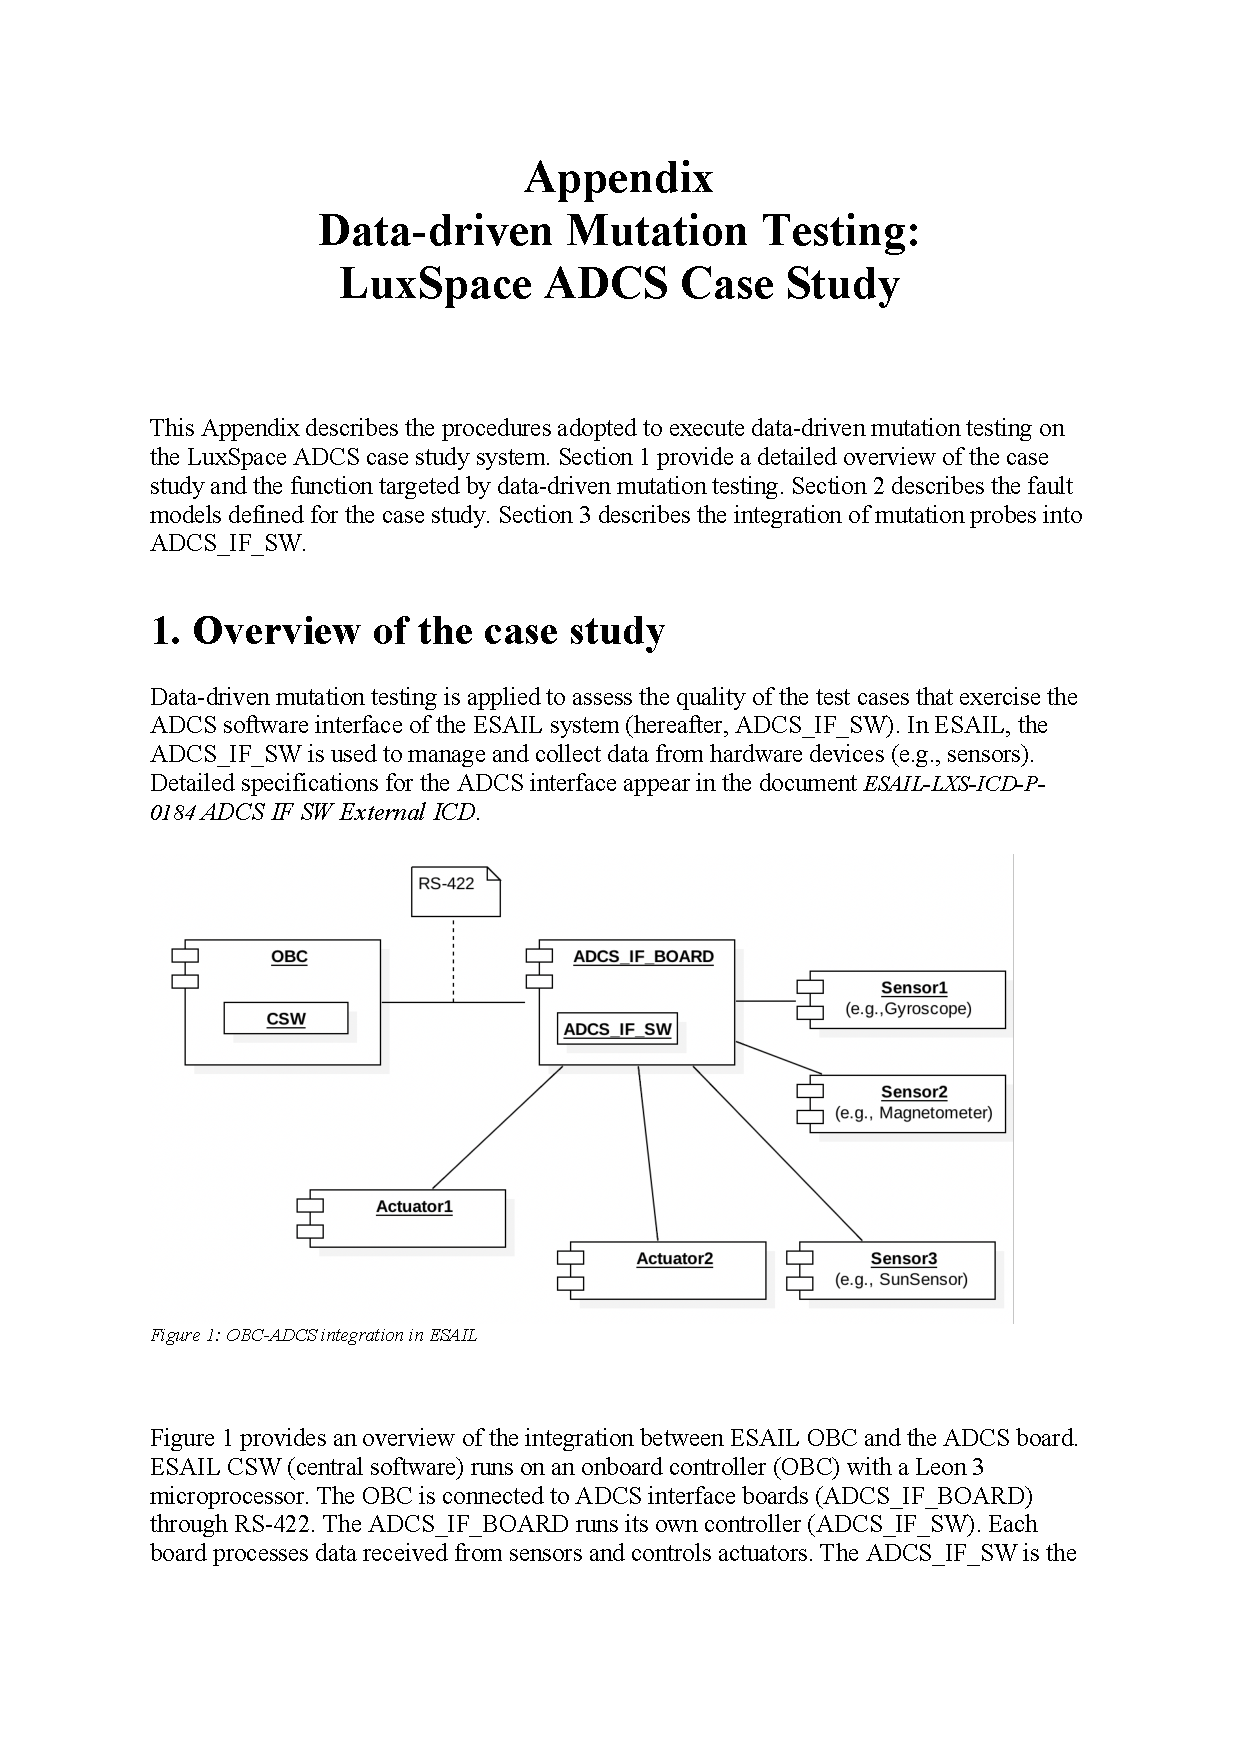
\includepdf[pages=-,scale=0.9,offset=0mm -75]{faultModels/ESAIL_ADCS_FaultModel_current_version.pdf}

   
%\clearpage
%% !TEX root = MAIN.tex
\chapter{ESA Revisions}

%% !TEX root = MAIN.tex

\section{Responses to ESA comments provided on 12.04.2021}
\label{sec:ESA:comments:1}

Comments IDs appear also in the main document next to the text modified to address the comment. To save space in the main text, the prefix \emph{ITSR-SSS-PABG-} has been abbreviated as \emph{P-}.

\setlength\LTleft{0pt}
\setlength\LTright{0pt}
\tiny 
%@{\extracolsep{\fill}}
\begin{longtable}{|p{1.5cm}|p{12cm}|@{}}
%\caption{\normalsize .}
%\label{table:comments:responses} 
\textbf{Comment ID}&\textbf{Response}\\
\\
\hline
P-1&
\begin{minipage}{12cm}
We will need to discuss the detail of the merge of the two specifications during the review meeting.
\end{minipage}\\
\\
\hline

P-2&
\begin{minipage}{12cm}
Done.
\end{minipage}\\
\\
\hline

P-3&
\begin{minipage}{12cm}
Done.
\end{minipage}\\
\\
\hline

P-4&
\begin{minipage}{12cm}
Done.
\end{minipage}\\
\\
\hline

P-5&
\begin{minipage}{12cm}
Done.
\end{minipage}\\
\\
\hline

P-6&
\begin{minipage}{12cm}
Done.
\end{minipage}\\
\\
\hline

P-7&
\begin{minipage}{12cm}
Done.
\end{minipage}\\
\\
\hline

P-8&
\begin{minipage}{12cm}
Done.
\end{minipage}\\
\\
\hline

P-9&
\begin{minipage}{12cm}
It is worth discussing if it makes sense to perform mutation analysis without code coverage.
\end{minipage}\\
\\
\hline


P-10&
\begin{minipage}{12cm}
We always generate all the mutants because it's fast. End-users have the option to execute a subset of them.
\end{minipage}\\
\\
\hline

P-11&
\begin{minipage}{12cm}
We changed a sentence, but this requirement is long because we had to provide an explanation missing from D2.
\end{minipage}\\
\\
\hline

P-12&
\begin{minipage}{12cm}
\end{minipage}\\
\\
\hline

P-13&
\begin{minipage}{12cm}
\end{minipage}\\
See P-8\\
\hline

P-14&
\begin{minipage}{12cm}
\end{minipage}\\
Action item. To be done for the end of WP3.\\
\hline


P-15&
\begin{minipage}{12cm}
TOD
\end{minipage}\\
\hline

P-16&
\begin{minipage}{12cm}
Done.
\end{minipage}\\
\hline

P-17&
\begin{minipage}{12cm}
We will provide a table for end of WP3.
\end{minipage}\\
\hline
                                                
\end{longtable}
\normalsize

\clearpage

% !TEX root = MutationTestingSurvey.tex

\section{Responses to ESA comments provided on 03.04.2020}
\label{sec:ESA:comments:2}


\setlength\LTleft{0pt}
\setlength\LTright{0pt}
\tiny 
\begin{longtable}{|p{1.5cm}|p{12cm}|@{}}
\label{table:comments:responses} 
\textbf{Comment ID}&\textbf{Comment and Response (below)}\\
\\
\midrule
C6 \& C7
&
Have you seen numbers for this mutation score and threshold in the literature? Is this something to be checked during the use case evaluation?
\\
\cmidrule{2-2}
&
We have addressed the comments above.
\TODO{OScar: please check if the survey of Papadakis say something aboth teh threshold (C7)}
\\
\hline
C8
&
Elaborate a bit more on C8 (pros and cons of doing mutation at source code / IR/ Assembly/ Executable);
\\
\cmidrule{2-2}
&
\TODO{Oscar: you may refer to taht paper of Darko Marinov and Co. to say IR is not good}
\\
\hline
C31
&
What is this sufficient set of operators?
\\
\cmidrule{2-2}
&
\TODO{Oscar}
\\
\hline
C32
&
Can you please add the solution for this example? i.e. do we need two different test cases of isPalindrome to detect both mutants?
\\
\cmidrule{2-2}
&
\TODO{Oscar}
\\
\hline
C33
&
Even if the objectives are complementary, both of them should be pursued for a data mutation testing approach?
\\
\cmidrule{2-2}
&
We have addressed the comment above.
\\
\hline
C34
&
The sentence sounds weird... To automate?? Is this activity something that can be automated?
\\
\cmidrule{2-2}
&
We have addressed the comment above by clarifying our text.
\\
\hline
C35
&
Is it possible to add an example of equivalent and redundant mutants?
\\
\cmidrule{2-2}
&
We have added the requested examples.
\\
\hline
C36
&
\begin{minipage}{12cm}
Related to automation, in my opinion, what it is key is that the test assessment process (for both data and code mutation) is as much automated as possible.\\

Automated generation of test cases is a very nice to have. In an industrial environment, let's say that we could afford spending some time to manually augment the test suite.\\

You may consider this to prioritize tasks within this activity.
\end{minipage}
\\
\cmidrule{2-2}
&
We agree on the comment. No need to change the text in this deliverable.
\\
\hline
C37
&
Are we missing a chapter to address the Generation of Test Oracles?\\
\cmidrule{2-2}
&
We have added a section concerning generation of test oracles for code-driven mutation testing (Section~\ref{sec:oraclesGeneration:codeDriven}) and data-driven mutation testing 
(Section~\ref{sec:oracles:dataMutation}).
\\
\hline
C38
&
\begin{minipage}{12cm}
a. From these Case Studies, is there any that you would like to try out within FAQAS?\\

b. One thing that we may need for FAQAS framework is to have kind of a test suite allowing to test the tool, and also to test the tool when new versions will be produced. Would any of these case studies fulfill that?
\end{minipage}
\\
\cmidrule{2-2}
&
We have discussed this topics by voice.
\\
\hline
C39
&
Do you have any information on the kind of test suite? (e.g. is it unit testing, system testing, ...)
\\
\cmidrule{2-2}
&
\TODO{}
\\
\hline
C40
&
Are these case studies focused on Code-Mutation, Data-Mutation, or both?\\
\cmidrule{2-2}
&
\TODO{}
\\
\hline
C41
&
Is there any meaningful conclusion (positive or negative) from those industrial case studies?\\
\cmidrule{2-2}
&
\TODO{}
\\
\hline
C42
&
\begin{minipage}{12cm}
Can we make a conclusion paragraph on this?\\

e.g. No tool based on mutation testing is known to be used within an industrial software development environment\\
e.g. Mutation testing is seen applied mainly within research environments\\
etc, etc
\end{minipage}
\\
\cmidrule{2-2}
&
\TODO{}
\\
\hline
C43
&
Is there any of these trends that could be meaningful to explore?
\\
\cmidrule{2-2}
&
\TODO{}
\\
\hline
C44
&
\begin{minipage}{12cm}
	\begin{itemize}
		\item Is there any particular trend for Code-Based mutation testing? (e.g. research is on-going or vanishing, the way to apply it, the type of operators used, the tools supporting it, ...)
		\item Any particular trend for Data-Based mutation testing?
	\end{itemize}
\end{minipage}
\\
\cmidrule{2-2}
&
\TODO{}
\\
\hline
C45&
\begin{minipage}{12cm}
D1 is fulfilling well requirement R1-1 as in the SoW. There is only one exception, on the red sentence below:\\

[R1-1.c] The applications of mutation testing (e.g. code and data mutation, test-suite evaluation, test cases generation, test-data generation, \textcolor{red}{code quality improvement}, ...)\\

The evaluation of code quality improvement is to be looked at. Indeed, this would be a secondary objective of applying mutation testing on space systems, but we would like to understand if mutation testing could help improve the code quality or not.\\
\end{minipage}
\\
\cmidrule{2-2}
&
\begin{minipage}{12cm}
We added a paragraph on Chapter~\ref{chapter:trends} explaining that there are no works in literature about quality code improvement based on code-driven mutation testing.
\end{minipage}
\\

\bottomrule                                                             
\end{longtable}
\normalsize

\clearpage


%\clearpage

\printindex

\bibliographystyle{IEEEtran}
\bibliography{bibliography}


\end{document}  